 \documentclass{article}

\usepackage{graphicx}
\usepackage[toc,page]{appendix}

\usepackage[a4paper]{geometry}
\usepackage[english]{babel}
\usepackage[T1]{fontenc}
\usepackage{hyperref}
\usepackage{amstext,amsmath,amsfonts}
\usepackage{dcolumn,booktabs}
\usepackage{color}
\usepackage{subfigure}
\usepackage{amsthm}

\makeatletter
\def\maketitle{%
  \null
  \thispagestyle{empty}%
  \vfill
  \begin{center}\leavevmode
    \normalfont
    {\LARGE \@title\par}%
    \vskip 1cm
    {\Large \@author\par}%
    \vskip 1cm
    {\Large \@date\par}%
  \end{center}%
  \vfill
  \null
  \cleardoublepage
  }
\makeatother
\title{Bachelor thesis}

\author{Kees ter Brugge\\}
                
                
\date{\today}

\begin{document}
 \maketitle



\newpage
Since we use two relatively small data sets to estimate the parameters of the unrestricted intrinsic bubble model, the estimates made by the nonlinear least squares regression might be biased. The used test statistics might not have the desired distribution when the distributions of the estimates are very skewed or have very fat tails and do not converge to the normal distribution. We can also see whether using the whole sample or the subsample yield has a large impact on the distributions of the estimates. We can evaluate the distribution of the estimates by means of a simulation. We generate a lot of data sets with chosen parameters and see what the distribution is of the estimates of those parameters.  \\

We first construct the log dividends series ${d_t}_{t=1871}^{2006}$ and ${d_t}_{t=1955}^{2006}$ as follows 
\begin{eqnarray}
d_t =  d_{t-1} + \epsilon_{t}
\end{eqnarray} 
where the $\epsilon_{t} \sim N(\mu, \sigma_\epsilon^2)$. With each dividends series we generate 500 price series ${P_t}_{t=1871}^{2006}$ and ${P_{t}}_{t=1955}^{2006}$ as follows
\begin{eqnarray}
P_t = c_0e^{d_t} + ce^{d_t\lambda} + \eta_t
\end{eqnarray}
where $\eta_t = 0.65 \eta_{t-1} -0.5 \eta_{t-2}+ 0.25 \eta_{t-3} $ . In figure (\ref{}) we can see that these values correspond to the partial autocorrelation coefficients of the residuals of the unrestricted intrinsic bubble model. Since the intrinsic bubble model did not produce white noise residuals but residuals that were autocorrelated, generating residuals as AR(3) processes produces prices series with a higher resemblance to the real prices series.

\begin{table}[h!]
\centering
\begin{tabular}{l|ll}   
parameter & 1871-2006 & 1955-2006 \\ \hline
$\mu$ & 0.016 & 0.020 \\
$\sigma_\epsilon$ & 0.126 & 0.050 \\
$d_0$ & 0.52& 1.72 \\
$c_0$ & 18.0 & 12.7 \\
c & 0.04 & 0.23 \\
$\lambda$ & 3.64 & 3.03 \\
$\sigma_\eta$ 7 & 11 \\  
\end{tabular}
\caption{d}
\label{d}
\end{table}
The parameters used in constructing these time series are estimates obtained by regressing log dividends as an random walk with drift and by the unrestricted intrinsic bubble model. 
 
The estimates of these parameters have the following distributions
\newpage
\begin{figure}[h]
	\centering
		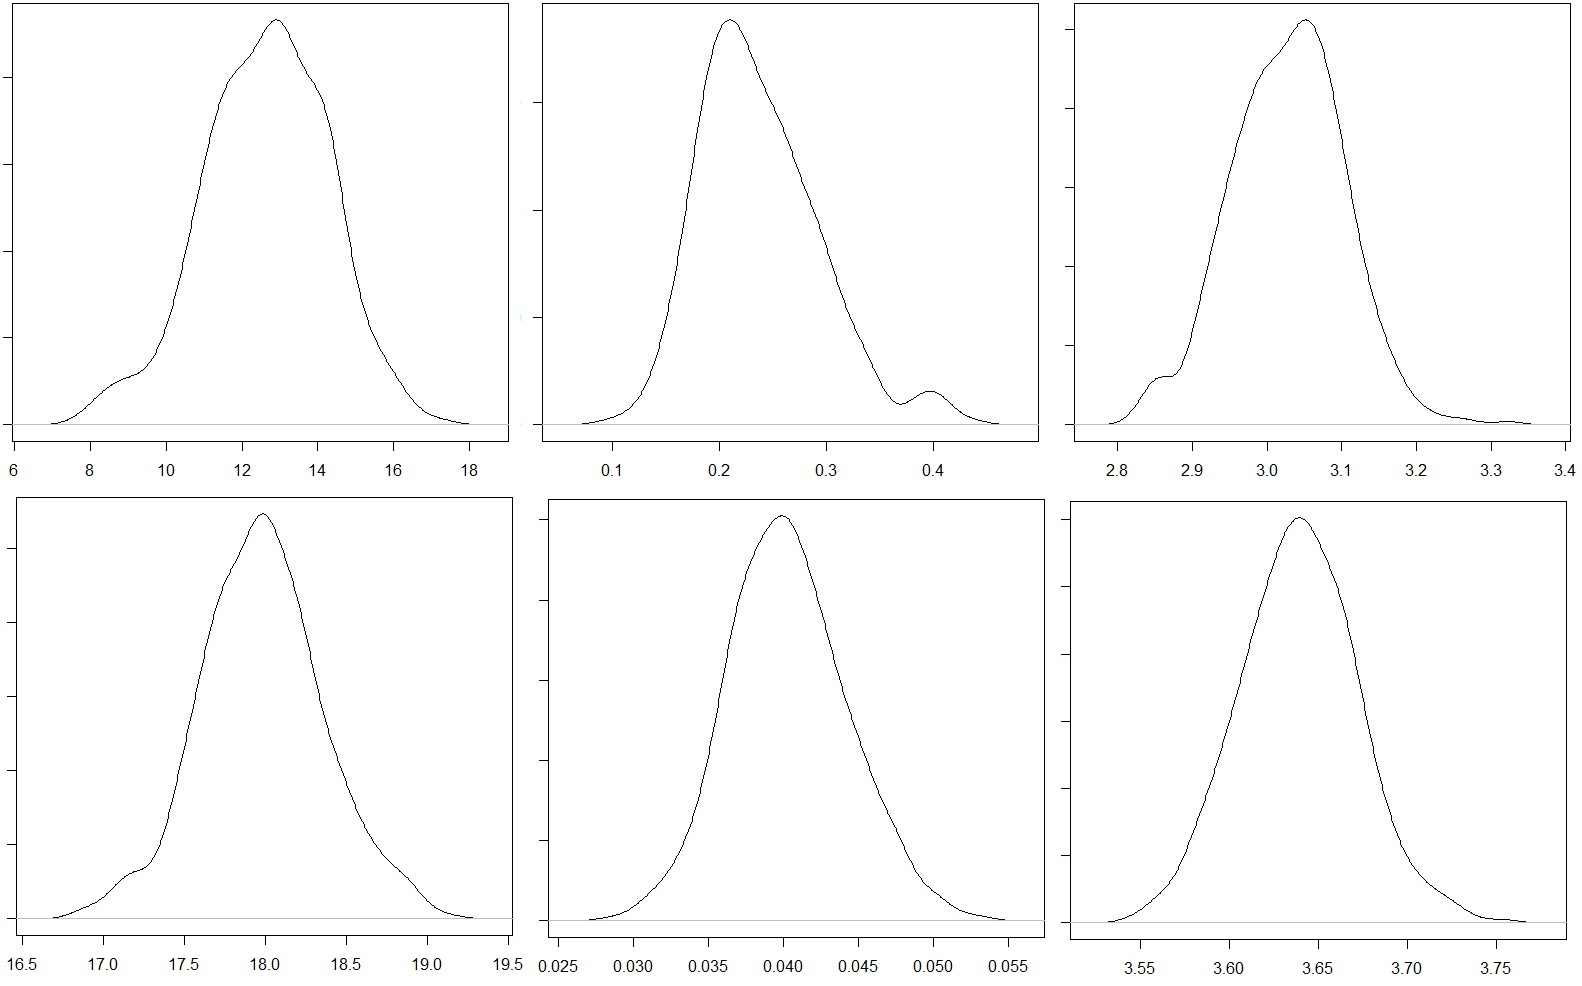
\includegraphics[width=0.99\textwidth]{C:/Users/kc/Downloads/distboth.jpg}
	\caption{Distribution of the estimates made by the intrinsic bubble model. Row one and two plot the distribution of the estimates produced by using the subsample and the whole sample respectively. The first, second and third column show the distribution of the estimates of $c_0, c$ and $\lambda$ respectively. }
	\label{simulation}
\end{figure}

In these plots we see that the distributions of the estimates approximate the normal distribution and are nicely centered around the real values of the parameters. The larger samples yields a less skewed  approximation of the normal distribution, but even with a sample size of 52 the approximation is quite good. 
\end{document}